\documentclass[a4paper]{article}
% Kodowanie latain 2
%\usepackage[latin2]{inputenc}
\usepackage[T1]{fontenc}
% Można też użyć UTF-8
\usepackage[utf8]{inputenc}
\usepackage{graphicx}

% Język
\usepackage[polish]{babel}
% \usepackage[english]{babel}
\usepackage{listings}

% Rózne przydatne paczki:
% - znaczki matematyczne
\usepackage{amsmath, amsfonts}
% - wcięcie na początku pierwszego akapitu
\usepackage{indentfirst}
% - komenda \url 
\usepackage{hyperref}
% - dołączanie obrazków
\usepackage{graphics}
% - szersza strona
\usepackage[nofoot,hdivide={2cm,*,2cm},vdivide={2cm,*,2cm}]{geometry}
\frenchspacing
% - brak numerów stron
\pagestyle{empty}

% dane autora
\author{Jakub Popiel, 323236}
\title{Sprawdzian \LaTeX}
\date{\today}

% początek dokumentu
\begin{document}
\maketitle


\section{Zad 1}
Przy pomocy komendy ssh-keygen wygenerowałem klucz, a następnie wrzuciłem go na  serwer przy pomocy ssh-copy-id, po czym zalogowałem się na serwer


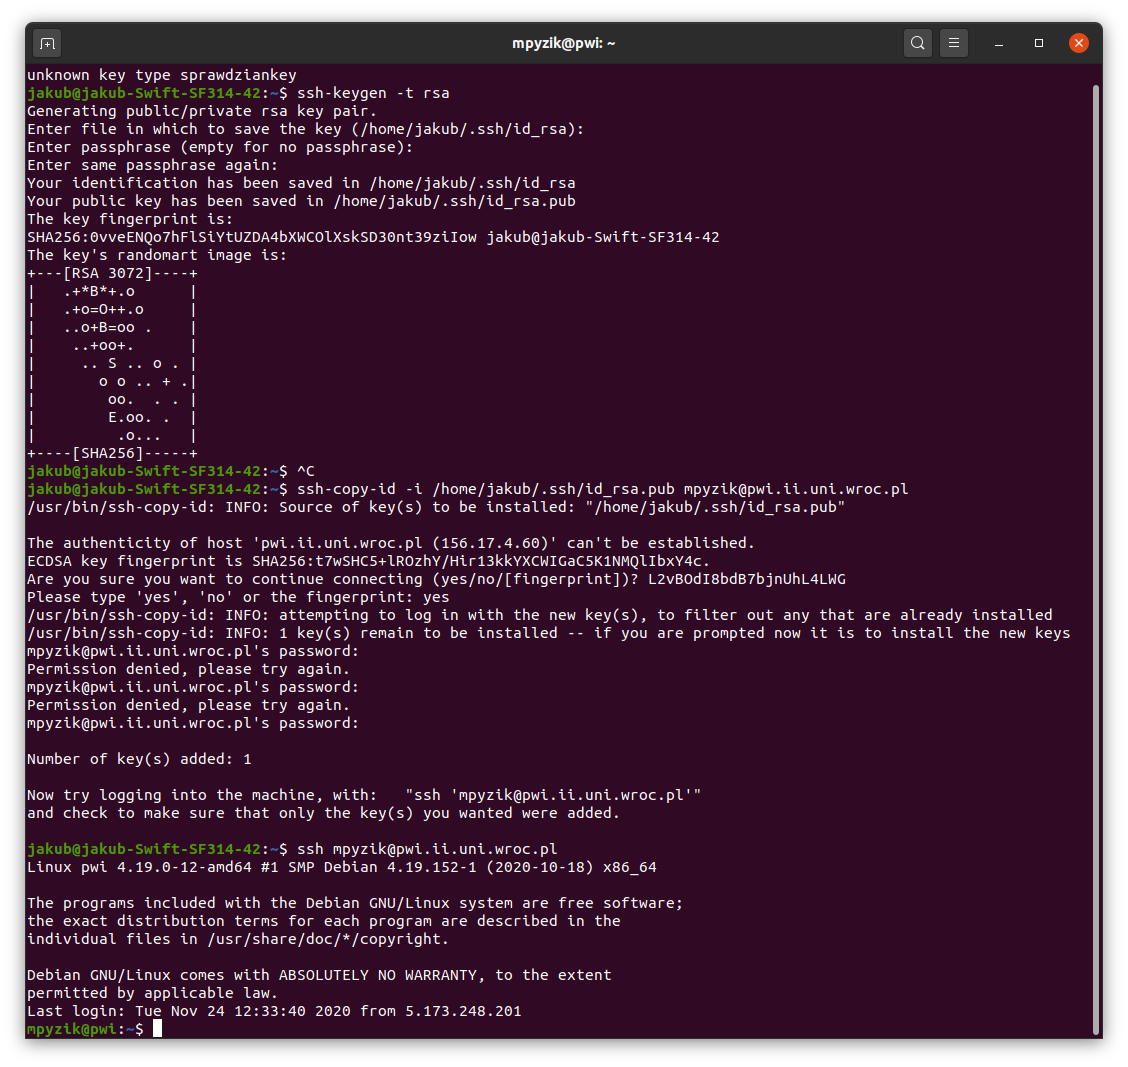
\includegraphics[scale=0.48]{Screenshot from 2020-11-24 12-34-56.png} 





\section{Zad 2}
Stworzyłem plik nazwany imieniem i nazwiskiem, a następnie dodałem do niego zadaną treść i wyświetliłem poleceniem less, po czym przeniosłem plik do nowo utworzonego katalogu "testy".

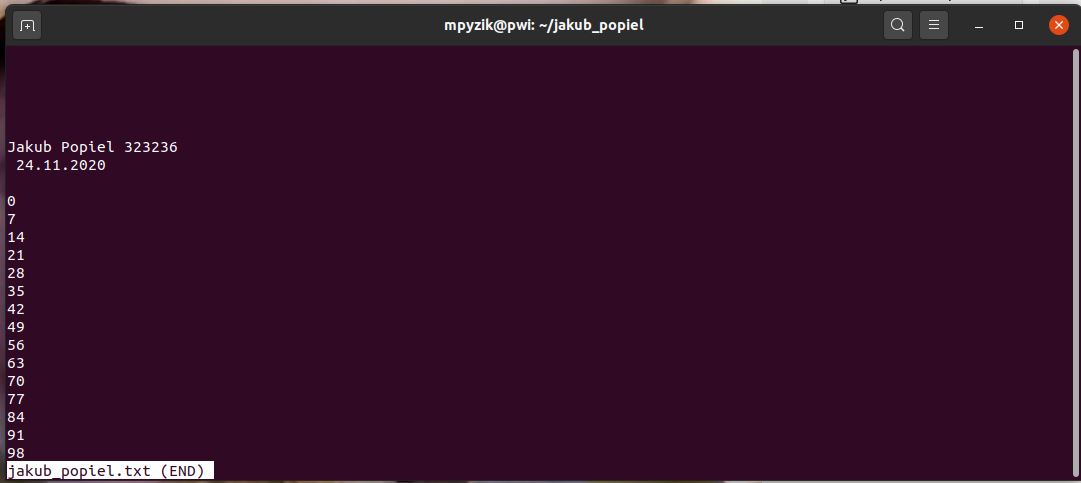
\includegraphics[scale=0.4]{Screenshot from 2020-11-24 12-51-07.png} 

Skorzystałem z następujących komend:
\begin{lstlisting}[language=bash]
  $ touch jakub_popiel.txt
  $ echo 'Jakub Popiel 323236' > jakub_popiel.txt
  $ echo ' 24.11.2020' >> jakub_popiel.txt
  $ seq 0 7 100 >> jakub_popiel.txt
  $ mkdir testy
  $ mv jakub_popiel.txt testy/
\end{lstlisting}

Następnie wylogowałem się z serwera i pobrałem plik do lokalnego katalogu przy pomocy komendy:

\begin{lstlisting}[language=bash] 
  $ scp -r mpyzik@pwi.ii.uni.wroc.pl:~/jakub_popiel/testy/jakub_popiel.txt .
\end{lstlisting}

\section{Zad 3}
Po powtórnym zalogowaniu na serwer przy pomocy wskazanej komendy stworzyłem 5 plików tekstowych, a następnie scaliłem je przy pomocy komendy cat.

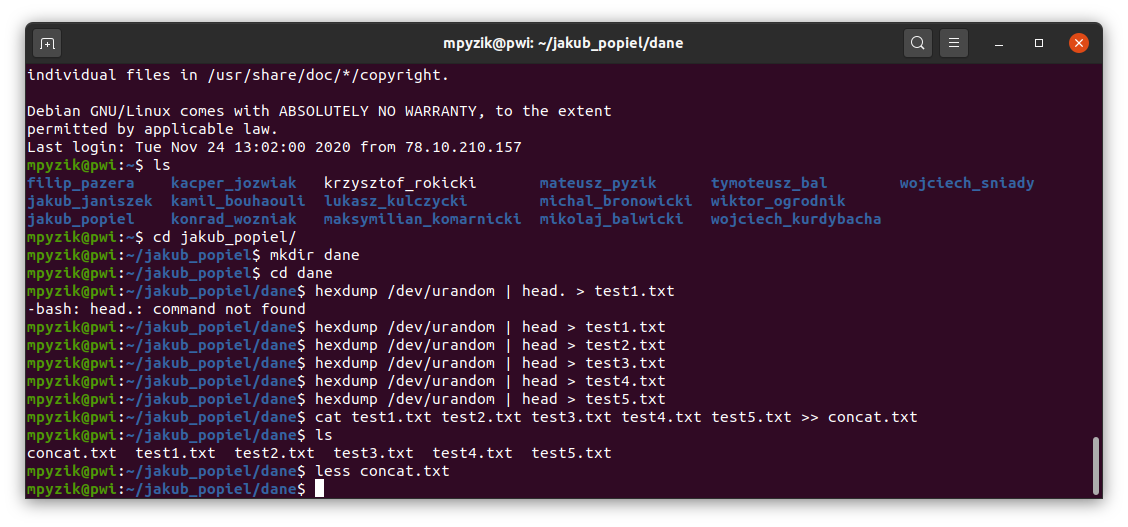
\includegraphics[scale=0.5]{Screenshot from 2020-11-24 13-09-51.png} 


\end{document}
